
% ----------------------------------------------------------
% PARTE
% ----------------------------------------------------------
\part{Preparação da pesquisa}

Este trabalho se baseia em um experimento quantitativo sobre problemas relacionados a segmentação e classificação de dados de uma base de dados grande, utilizando algoritmos de K médias, regressão logística e random forest. Serão feitas interpretações, análises e comparações, levantando aspectos positivos e negativos de cada metodologia.

\begin{landscape}
\centering
\begin{vplace}[0.7]
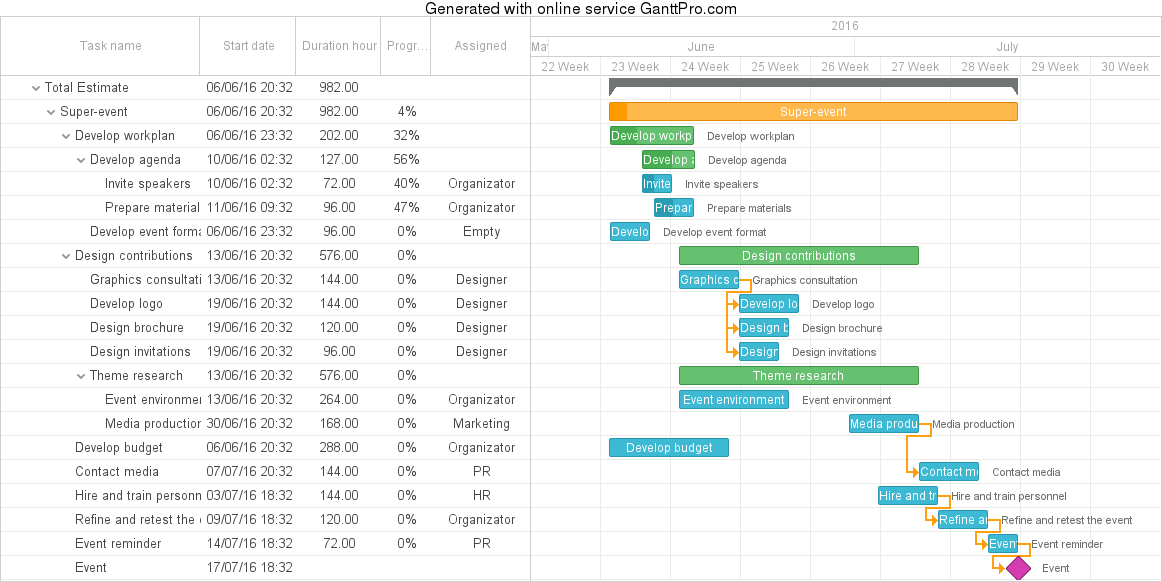
\includegraphics[width=\textwidth]{gantt}
\end{vplace}
\end{landscape}

% ----------------------------------------------------------
